\documentclass{article}
\usepackage[french]{babel}
\usepackage[T1]{fontenc}

\usepackage{graphicx} % Required for inserting images
\graphicspath{{C:/Users/chabe/Documents/L3/PROJET/Projet/CRFinal/ressources/}}
\usepackage{amsmath}
\usepackage{amsfonts}
\usepackage{tikz}
\usepackage{fancyhdr}
\usepackage{thmbox}

\pagestyle{fancy}
\fancyhead{}
\fancyfoot{}
\fancyhead[L]{Attracteur de Lorenz - \thesection}
\fancyfoot[C]{\thepage}

\title{Système de Lorenz}


\newcommand*\colv[1]{
\left(\begin{array}{c}
    #1
\end{array}\right)
}

\newcommand{\R}{\mathbb{R}}

\newcommand{\deriv}[3][ ]{
    \ensuremath{\frac{\mathrm{d}^{#1}#2}{\mathrm{d}^{#1} #3}}
}
\newcommand{\id}[1][]{\ensuremath{\mathrm{Id}_{#1}}}

\newcommand{\cad}{c'est-\`a-dire }

\newtheorem[M]{prop}{Proposition}[section]
\newtheorem[M]{propt}{Propriété}[section]
\newtheorem[L]{thm}{Théoreme}
\newtheorem[L]{cor}{Corollaire}

\begin{document}
\begin{titlepage}
    \vfil
    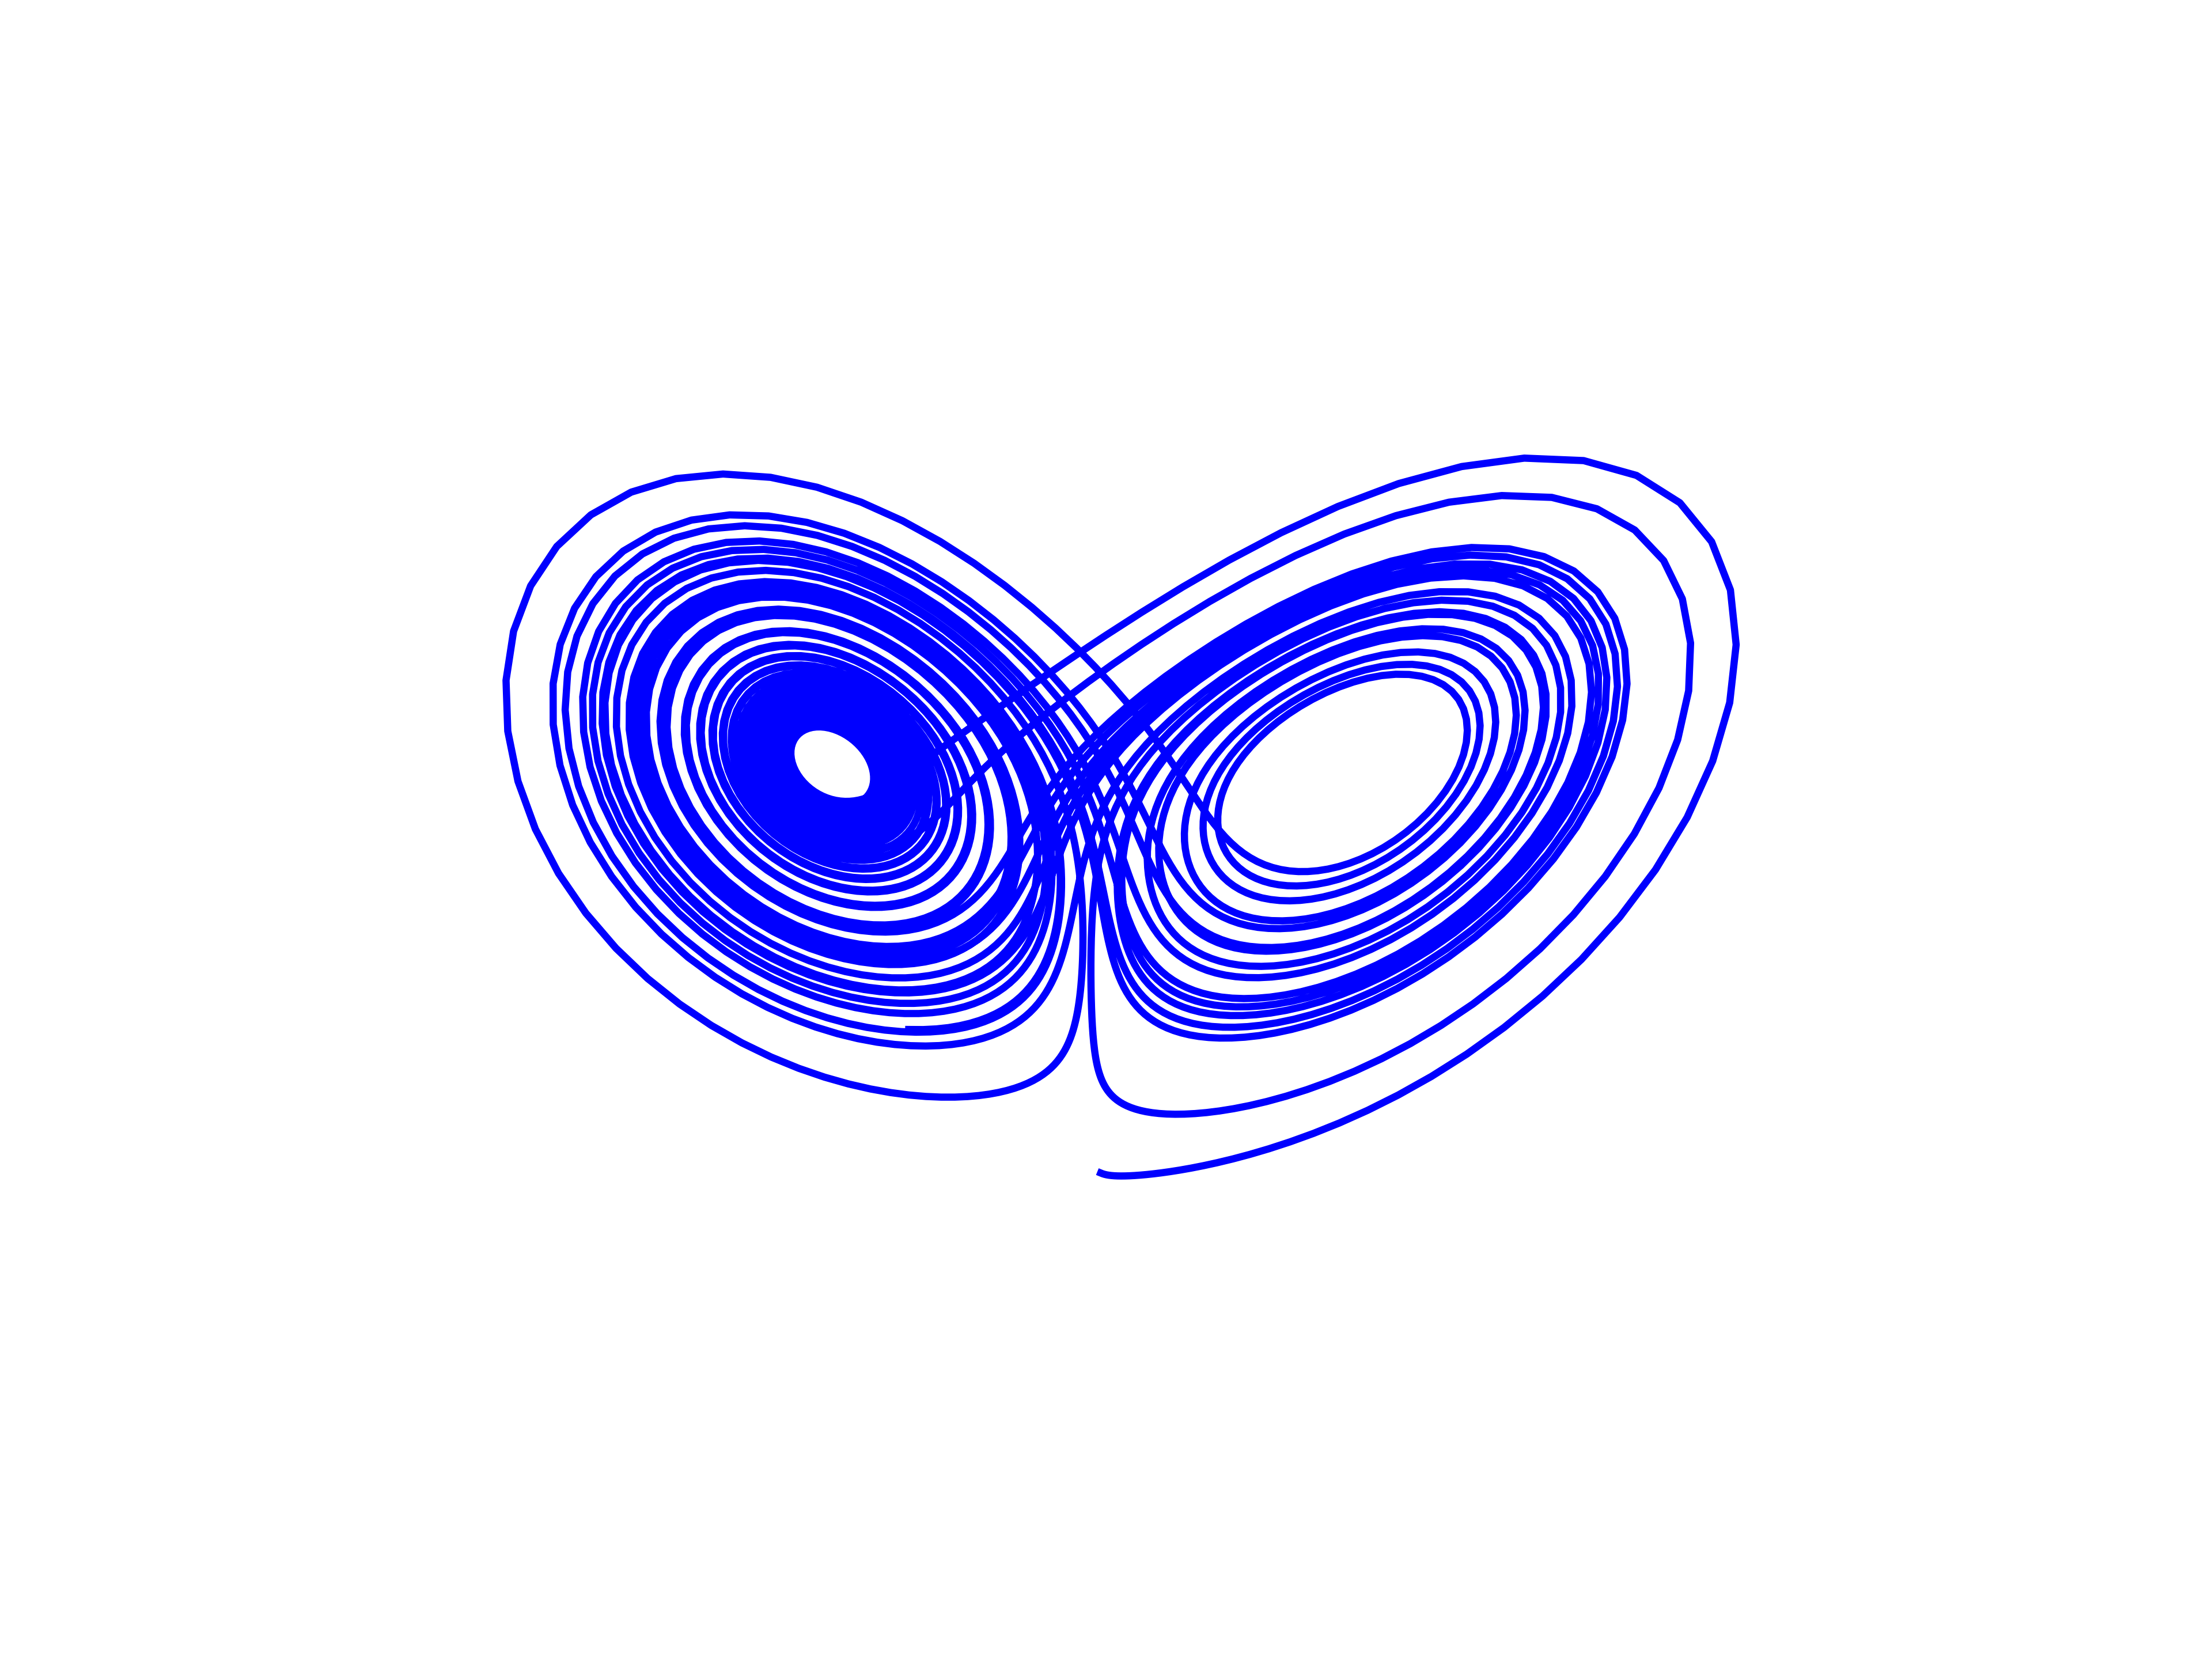
\includegraphics{LorenzTransparent}
\end{titlepage}
\section*{Introduction}

\begin{equation}
    \label{Lorenz}
    \left\{
    \begin{array}{rl}
        x' &=\sigma(y-x) \\
        y' &=\rho x -y - xz\\
        z' &=xy - \beta z
    \end{array}
    \right.
    \begin{array}{r}
        (L_1)\\
        (L_2)\\
        (L_3)
    \end{array}
\end{equation}

\begin{equation}
    \label{fLorenz}
    \deriv{\Vec{u}}{t} = \Gamma(\Vec{u}), \quad
    \Gamma : \Vec{u} = \colv{x\\y\\z} \in \R^3 \mapsto \colv{\sigma(y-x) \\ \rho x-y-xz \\ xy-\beta z}
    \end{equation}

\section{Méthodes numériques}


\section{Existence et première propriété}

Dans cette section nous allons faire une étude du systeme de Lorenz afin de determiner l'existence des solutions. Nous nous limiterons à l'étude des temps positifs ($t \ge 0$)

\begin{prop}
    Le systeme de Lorenz admet des solutions. De plus les solutions sont globales sur $\R_+$ et de classe $C^1$
\end{prop}

\begin{proof}
    $\Gamma$ est $C^1$ donc elle est localement Lipschitzienne, de plus elle de depend pas directement du temps. D'après le théoreme de Cauchy-Lipschitz, l'équation \eqref{Lorenz} admet une unique solution maximale de classe $C^1$ que l'on notera $(I,(x,y,z))$ avec $I \subset \R_+$ avec $I = [0,T[,\ T \in ]0,+\infty]$. Montrons que $(I,(x,y,z))$ est globale. Dans \eqref{Lorenz} on s'intéresse à la somme de, $x$ fois première ligne avec $y$ fois la seconde ligne et $z$ fois la troisième ligne.
\[
    xx'+yy'+zz' = \sigma yx - \sigma x^2 + \rho xy - y^2 -xyz + xyz - \beta z^2\\
\]  
Posons $\mathcal{N}: (t) \in \R^3 \mapsto x(t)^2 + y(t)^2 + z(t)^2$ ($\mathcal{N}$ est la norme euclidienne au carré)

\begin{align*}
    \Rightarrow \frac{1}{2}\deriv{ }{t}\mathcal{N}(t) & =(\sigma + \rho)x(t)y (t) -\sigma x^2(t) - y^2(t) - \beta z^2(t)\\
    & \le (\sigma + \rho)x(t)y(t) +\min (1,\sigma,\beta)\mathcal{N}(t)\\
    & \le (\frac{\sigma+\rho}{2})(x^2(t) + y^2(t)) +\min (1,\sigma,\beta) \mathcal{N}(t) &&\mathit{(Young)}\footnotemark \\
    & \le (\frac{\sigma+\rho}{2})(x^2(t) + y^2(t) + z^2(t)) +\min (1,\sigma,\beta) \mathcal{N}(t)\\
    & \le \bigg[\frac{\sigma + \rho}{2} + \min (1,\sigma,\beta) \bigg] \mathcal{N}(t)
\end{align*}
\footnotetext{$\forall p,q \in \mathbb{N}\: \text{tels que} \frac{1}{p}+\frac{1}{q}=1 \Rightarrow \forall a,b \in \R \: ab \le \frac{a^p}{p}+\frac{b^q}{q}$}

Posons $ \eta = \sigma + \rho - 2 \min (1,\sigma,\beta))$. On a alors: 
\[
    \forall t \in \R_+, \  \deriv{}{t}\mathcal{N}(t) \le \eta\  \mathcal{N}(t)
\]
D'après le lemme de Grönwall il vient:
\[
    \forall t \in \R_+,\  \mathcal{N}(t) \le \mathcal{N}_0 e^{\eta t},\  \textrm{avec } \mathcal{N}_0 = \mathcal{N}(0)
\]
Donc la norme du vecteur solution n'explose pas en temps fini.
\end{proof}

En ayant obtenue les résultats de la proposition on peut aisément en déduire que la propriété suivante.

\begin{propt}
    Les solutions du système de Lorenz \eqref{Lorenz} sont de classe $C^\infty$
\end{propt}

\begin{proof}
    Par \eqref{fLorenz} on a que $(x',y',z') = \Gamma(x,y,z)$, or par composition $\Gamma(x,y,z)$ est $C^1$ donc $(x',y',z')$ l'est aussi, ainsi $(x,y,z)$ est $C^2$.De la même manière on obtient par récurence immédiate que $(x,y,z)$ est $C^\infty$
\end{proof}

Cette propriété nous permet de dire que même si \eqref{Lorenz} est un système dit chaotique, on peut affirmer que les solutions sont régulière.

\section{\'Etude des points stationnaires}
Après une première etude sommaire du système de Lorenz \eqref{Lorenz}, on s'intéresse maintenant à l'étude des points stationnaires. Les points stationnaires sont des points tels que si le système passe par un de ces points il y reste indéfiniment.

%vérifier la formulation de ce théoreme
\begin{thm}
    $u' = f(u)$ si il existe $v$ tel que $f(v)=0$ alors $v$ est un point stationnaire de l'équation differentielle.
\end{thm}

\subsection{Rappel des théorèmes}
\label{sec:Rappel-des-théorèmes}
D'abord on rappelle les résultats sur lesquels on s'appuiras dans la suite. Ces théorèmes établissent des résultats de stabilité sur les point stationnaires en se basant sur l'étude spectrale de la differentielle.
\begin{thm}
    \label{thm:eq-ass-stable}
    Soit $f\in C^2(U;E)$ sur un ouvert $U$ d'un espace de Banach $E$ et $v\in U$ tel que $f(v)=0$. Si le spectre de $\mathcal{D}_\Gamma(v)$ est inclus dans le demi-plan ouvert $\left\{\lambda; \Re(\lambda)<0\right\}$ alors $v$ est un point d'équilibre assymptotiquement stable pour l'équation $u'=f(u)$
\end{thm}

Ce résultat nous permet de conclure sur le comportement assymtotique des solutions ayant subit une faible perturbation à l'instant de départ (\cad les solution $(\R_+,u_1)$ telles que $u_1(t_{\text{init}})=u(t_{\text{init}})+\varepsilon,\ 0<\|\varepsilon\|\ll 1 $ ). On obtient ainsi $\lim_{t\to\infty}\|u-u_1\| = 0$.

%resultat pour la stabilité simple

\begin{thm}
    \label{thm:eq-instable}
    Soit $f\in C^2(U;E)$ et $v\in U$ tel que $f(v)=0$. Si $\max\{\Re(\lambda); \lambda\in \mathrm{Sp}(\mathcal{D}_f(v))\}$ est atteint pour une valeur propre de $\mathcal{D}_f(v)$ de partie réelle strictement positive. Alors $v$ est un point d'équilibre instable pour l'équation $u'=f(u)$
\end{thm}

% commentaire sur le résultat

\subsection{Détermination des équilibres}
Dans un premier temps on regarde si notre système possèdes des équilibres et si oui lesquels.
\begin{prop}
    L'equation \eqref{Lorenz} possèdes 3 points d'équilibre qui sont:
    \begin{align*}
        0_{\R^3} &&   S_+ :=\colv{\sqrt{ \beta (\rho -1)} \\ \sqrt{\beta (\rho -1)}\\ \rho -1}  &&  S_- := \colv{-\sqrt{ \beta (\rho -1)} \\ - \sqrt{\beta (\rho -1)}\\ \rho -1}
    \end{align*}
\end{prop}

\begin{proof}
On remarque que $(0,0,0)$ est un point stationnaire, en effet $\Gamma(0,0,0) = 0_{\R^3}:= 0$ donc ($\R_+$,0) est une solution de l'equation differentielle.\\
On resout alors $\Gamma(x,y,z)=0$ en supposant que $(x,y,z) \neq 0$, il vient:
\[
\left\{\begin{array}{rl} %O of Gamma
     \sigma(y-x)&=0  \\
     \rho x -y -xz&=0\\
     xy - \beta z&=0
\end{array}\right.
\begin{array}{c} %Num eq
    (L_1)\\
    (L_2)\\
    (L_3)
\end{array}
\]
de $(L_1)$ on obtient que $x=y$. Dans $(L_2)$ et dans $(L_3)$ on remplace $y$ par $x$, il vient alors:
\begin{gather*}
    (L_2) \Rightarrow \rho x - x - xz = 0 \Rightarrow x (\rho -1 -z ) = 0 \\
    (L_3) \Rightarrow x^2 - \beta z = 0 \Rightarrow z = \frac{x^2}{\beta}
\end{gather*}
On obtient ainsi un polynome de degrès 3 il y a donc au plus 3 équilibres:
\begin{align*}
    (L_2) & \Rightarrow x (\rho - 1 - \frac{x^2}{\beta}) = 0 \text{, or }x \neq 0\\
        & \Rightarrow x^2 = \beta (1-\rho)\\
    \text{Si } \beta(1-\rho) \ge 0 & \Leftrightarrow \beta \ge 0,\rho\le 1 \text{ ou } \beta \le 0,\rho\ge 1\text{ alors:}\\
    &\Rightarrow x = \pm \sqrt{\beta(1-\beta)}
\end{align*}

De ces trois équation on obtient que:
\[
    \Gamma(x,y,z)=0_{\R^3} \Rightarrow (x,y,z) = (\pm \sqrt{ \beta (\rho -1)} ,\pm \sqrt{\beta (\rho -1)}, \rho -1)
\]

On verifie aisément que cette relation est une \'equivalance, en ramplacant les valeurs obtenue de $x$,$y$ et $z$ dans $\Gamma(x,y,z)$
\end{proof}

\begin{example}[Remarque]
    Si $\rho=1$ il n'y a qu'un seul équilibre.
\end{example}

\subsection{Caractérisation de l'équilibre $0_{\R^3}$}
Afin d'utiliser les outils introduit dans la partie \ref{sec:Rappel-des-théorèmes}, on calcule le polynome caractéristique de la differentielle en $0$ (noté $\chi$) donné par le calcul suivant.
\[
    \chi (\lambda) = \det\big(\lambda\id - \mathcal{D}_{\Gamma}(0,0,0)\big) = (\lambda - \beta)(\lambda^2 + \lambda(\sigma+1)+\sigma-\rho\sigma)
\]
\begin{example}[Remarque]
    $\beta$ est toujours racine de $\chi$
\end{example}
On remarque que $\chi$ est un polynome de degrè 3 et d'après la remarque précédente on a que $\chi(\lambda) = (\lambda - \beta)P(\lambda)$, avec $P:\lambda \in \R \mapsto \lambda^2 + \lambda(\sigma+1)+\sigma-\rho\sigma$. Ainsi les pour étudier $\chi$, on calcule le deteterminant de $P$:
\[
  \Delta = (\sigma+1)^2 - 4(\sigma-\sigma\rho)) = (\sigma-1)^2 +4\sigma\rho
\]

\begin{prop}[Cas 1:]
Si $(\rho,\sigma)=(0,1)$, alors: 
\begin{enumerate}
    \item Si $\beta > 0$ alors 0 équilibre instable pour \eqref{Lorenz}
    \item Si $\beta < 0$ alors 0 équilbre asymptotiquement stable pour \eqref{Lorenz}
\end{enumerate}
\end{prop}
\begin{proof}
    Dans ce cas on a, $\chi(x) = (\lambda-\beta)(\lambda+1)^2$. Donc $\mathrm{Sp} (\mathcal{D}_\Gamma(0,0,0))= \{ \beta, -1 \}$, on différencie alors 2 cas. Si $\beta$ est strictement positif alors d'après \ref{thm:eq-instable} l'équilibre est instable. Si $\beta$ est strictement négatif d'après \ref{thm:eq-ass-stable} l'équilibre est assymptotiquement stable
\end{proof}

\underline{Cas 2: Si $(\rho,\sigma)=(1,-1)$:}\\
Alors $\chi_A(\lambda) = (\lambda-\beta)\lambda^2$, donc d'après le théoreme, si $\beta$ est strictement positif (resp. strictement négatif) $0_{\R^3}$ est un point d'équilibre instable (resp. asymptotiquement stable) pour \eqref{Lorenz}


\underline{Cas 3: Si $\rho \in ]0,1[, \sigma \in \mathbb{R}$:}\\
$\Delta> (\sigma-1)^2 >0$ donc $P$ a deux racines réelles.
que l'on note: 
\[
    \lambda_\pm = \frac{-(\sigma-1)\pm \sqrt{(\sigma-1)^2 + 4\sigma\rho}}{2}
\]
Regardons le signe des racines. $\lambda_+ < -(\sigma-1)+ \sqrt{(\sigma+1)^2} \le 0 $, de même pour $\lambda_-$, on a, $\lambda_- < - \sigma +1- |\sigma - 1| \le 0$. De plus si $\beta$ est strictement négatif, toutes les racines sont strictement négative donc $0_{\R^3}$ est un point d'équilibre asymptotiquement stable pour \eqref{Lorenz}. Si $\beta > 0$, $0_{\R^3}$ est un point d'équilbre instable.

\underline{Cas 4: Si $\rho > 1$ et $\sigma \ge 0 $: }\\
Dans ce cas on a $\Delta > 0$, on retrouve la même expression des racines que précédemment $\lambda_\pm$. On trouve que $2\lambda_+ > 1-\sigma+|\sigma+1| \ge 0$, donc $\lambda_+ > 0$, pour $\lambda_-$ on a, $2\lambda_- < 1-\sigma-|\sigma+1| \le 0 $, donc $\lambda_- < 0$, dans ce cas $0_{\R^3}$ est un équilibre instable pour \eqref{Lorenz}.

\underline{Cas 5: Si $\rho<0$ et $\sigma\le 0$:}\\
Comme dans le cas précédent on trouve $\Delta>0$ avce cette fois $\lambda_+ < 0$ et $\lambda_- >0$. On le retrouve en majorant $2\lambda_+$ et $2\lambda_-$ par $\rho=0$, on majore ainsi $\lambda_+$ et minore $\lambda
_-$. Donc $0_{\R^3}$ est un équilbre instable pour \eqref{Lorenz}.

\subsection{Caractérisation de $S_\pm$}
\section{Annexes}


\end{document}